% This is "sig-alternate.tex" V2.1 April 2013
% This file should be compiled with V2.5 of "sig-alternate.cls" May 2012
%
% This example file demonstrates the use of the 'sig-alternate.cls'
% V2.5 LaTeX2e document class file. It is for those submitting
% articles to ACM Conference Proceedings WHO DO NOT WISH TO
% STRICTLY ADHERE TO THE SIGS (PUBS-BOARD-ENDORSED) STYLE.
% The 'sig-alternate.cls' file will produce a similar-looking,
% albeit, 'tighter' paper resulting in, invariably, fewer pages.
%
% ----------------------------------------------------------------------------------------------------------------
% This .tex file (and associated .cls V2.5) produces:
%       1) The Permission Statement
%       2) The Conference (location) Info information
%       3) The Copyright Line with ACM data
%       4) NO page numbers
%
% as against the acm_proc_article-sp.cls file which
% DOES NOT produce 1) thru' 3) above.
%
% Using 'sig-alternate.cls' you have control, however, from within
% the source .tex file, over both the CopyrightYear
% (defaulted to 200X) and the ACM Copyright Data
% (defaulted to X-XXXXX-XX-X/XX/XX).
% e.g.
% \CopyrightYear{2007} will cause 2007 to appear in the copyright line.
% \crdata{0-12345-67-8/90/12} will cause 0-12345-67-8/90/12 to appear in the copyright line.
%
% ---------------------------------------------------------------------------------------------------------------
% This .tex source is an example which *does* use
% the .bib file (from which the .bbl file % is produced).
% REMEMBER HOWEVER: After having produced the .bbl file,
% and prior to final submission, you *NEED* to 'insert'
% your .bbl file into your source .tex file so as to provide
% ONE 'self-contained' source file.
%
% ================= IF YOU HAVE QUESTIONS =======================
% Questions regarding the SIGS styles, SIGS policies and
% procedures, Conferences etc. should be sent to
% Adrienne Griscti (griscti@acm.org)
%
% Technical questions _only_ to
% Gerald Murray (murray@hq.acm.org)
% ===============================================================
%
% For tracking purposes - this is V2.0 - May 2012


\documentclass{sig-alternate-05-2015}

\usepackage{ragged2e}

\begin{document}

% Copyright
%\setcopyright{}
%\setcopyright{acmlicensed}
%\setcopyright{rightsretained}
%\setcopyright{usgov}
%\setcopyright{usgovmixed}
%\setcopyright{cagov}
%\setcopyright{cagovmixed}


% DOI
%\doi{10.475/123_4}

% ISBN
%\isbn{}

%Conference
%\conferenceinfo{PLDI '13}{June 16--19, 2013, Seattle, WA, USA}
\acmPrice{\$-24.32}

%
% --- Author Metadata here ---
%\conferenceinfo{WOODSTOCK}{'97 El Paso, Texas USA}
%\CopyrightYear{2007} % Allows default copyright year (20XX) to be over-ridden - IF NEED BE.
%\crdata{0-12345-67-8/90/01}  % Allows default copyright data (0-89791-88-6/97/05) to be over-ridden - IF NEED BE.
% --- End of Author Metadata ---

\title{FemtoGraph: A Pregel Based Shared-memory Graph Processing Library}
\subtitle{[Extended Abstract]}
%
% You need the command \numberofauthors to handle the 'placement
% and alignment' of the authors beneath the title.
%
% For aesthetic reasons, we recommend 'three authors at a time'
% i.e. three 'name/affiliation blocks' be placed beneath the title.
%
% NOTE: You are NOT restricted in how many 'rows' of
% "name/affiliations" may appear. We just ask that you restrict
% the number of 'columns' to three.
%
% Because of the available 'opening page real-estate'
% we ask you to refrain from putting more than six authors
% (two rows with three columns) beneath the article title.
% More than six makes the first-page appear very cluttered indeed.
%
% Use the \alignauthor commands to handle the names
% and affiliations for an 'aesthetic maximum' of six authors.
% Add names, affiliations, addresses for
% the seventh etc. author(s) as the argument for the
% \additionalauthors command.
% These 'additional authors' will be output/set for you
% without further effort on your part as the last section in
% the body of your article BEFORE References or any Appendices.

\numberofauthors{2} %  in this sample file, there are a *total*
% of EIGHT authors. SIX appear on the 'first-page' (for formatting
% reasons) and the remaining two appear in the \additionalauthors section.
%
\author{
% You can go ahead and credit any number of authors here,
% e.g. one 'row of three' or two rows (consisting of one row of three
% and a second row of one, two or three).
%
% The command \alignauthor (no curly braces needed) should
% precede each author name, affiliation/snail-mail address and
% e-mail address. Additionally, tag each line of
% affiliation/address with \affaddr, and tag the
% e-mail address with \email.
%
% 1st. author
  \alignauthor
  Alex Ballmer\\
       \affaddr{Illinois Institute of Technology}\\
       \email{alexandersballmer@gmail.com}
       \alignauthor
       Ioan Raicu\\
       \affaddr{Illinois Institute of Technology}\\
       \email{iraicu@cs.iit.edu}
}
% There's nothing stopping you putting the seventh, eighth, etc.
% author on the opening page (as the 'third row') but we ask,
% for aesthetic reasons that you place these 'additional authors'
% in the \additional authors block, viz.
%\additionalauthors{Additional authors: John Smith (The Th{\o}rv{\"a}ld Group,
%email: {\texttt{jsmith@affiliation.org}}) and Julius P.~Kumquat
%(The Kumquat Consortium, email: {\texttt{jpkumquat@consortium.net}}).}
%\date{30 July 1999}
% Just remember to make sure that the TOTAL number of authors
% is the number that will appear on the first page PLUS the
% number that will appear in the \additionalauthors section.

\maketitle
\begin{abstract}
  \justify
  The emerging applications for large graphs in big data science and social networks has led to the development of numerous parallel or distributed graph processing applications. The need for faster manipulation of graphs has driven the need to scale accross large core counts and many parallel machines. While distributed memory parallel systems continue to be used for high performance computing, some smaller systems make use of shared memory (SMP) and larger core counts. I hope to explore ways to utilize these larger shared memory systems by implementing a framework for manipulating graphs at a large scale. This system should be able to leverage and scale to very large core counts and provide a framework for later incorporating distributed processing across multiple nodes.
\end{abstract}


% The code below should be generated by the tool at
% http://dl.acm.org/ccs.cfm
% Please copy and paste the code instead of the example below. 
%
\begin{CCSXML}
  <ccs2012>
  <concept>
  <concept_id>10003752.10003809.10010170.10010171</concept_id>
  <concept_desc>Theory of computation~Shared memory algorithms</concept_desc>
  <concept_significance>500</concept_significance>
  </concept>
  </ccs2012>
\end{CCSXML}

\ccsdesc[500]{Theory of computation~Shared memory algorithms}
%
% End generated code
%

%
%  Use this command to print the description
%
\printccsdesc

% We no longer use \terms command
%\terms{Theory}

\keywords{Graph processing; Parallel Algorithms; Shared Memory}

\section{Introduction}
\justify
I propose a graph processing application, FemtoGraph, which will use a vertex-centric approach. This approach involves calling a function in the context of a vertex for each and every vertex. This function can modify or read from edges and other vertices.  Computation occurs in intervals or steps, with some form of communication between steps. Vertex-centric algorithms can be either synchronous, meaning every vertex function must finish before the next step begins, or asynchronous, which means that the next step can begin in the context of one vertex immediately.  \cite{Gz:7}

FemtoGraph is based off of the pregel model. Pregel is a vertex-centric graph processing model. Pregel is synchronous, with computation occurring in steps called supersteps. There is a messaging system for sending data and state to vertices in the next superstep, but not to any vertex in the current superstep. Vertices can do computations, modify neighbor vertices and edges, send messages to vertices in the next superstep, and vote to halt, meaning it cannot run its compute function until it receives a message or all vertices have voted to halt. When all vertices have voted to halt, the simulation ends. \cite{Gz:4}

\section{Related Work}
\justify
One of the main similar applications in this area is GraphLab. GraphLab is another vertex-centric graph processing framework that can either run on a single node using shared memory, or as a distributed application. GraphLab is the simplest to compare to FemtoGraph as it can run with shared memory without the harsh overhead of frameworks like Hadoop or Spark. GraphLab is asynchronous, which gives it the edge of not having to wait for the fist superstep to complete before starting the next superstep. \cite{Gz:6} Graphlab was the main point of comparison of FemtoGraph 


\section{Implementation}
\justify
FemtoGraph is implemented in C++ using parts of the Boost C++ library. There are 3 main parts. Vertex storage, the message queue, and the compute function. Vertex storage also stores edges and uses  an adjacency list using C++ vectors. The message queue is implemented using boost lockless queues, one for each vertex. The compute function is a user defined function that is run in the context of each vertex during a pregel superstep. Update functions are called in parallel with a user defined number of threads.

\section{Problem}
\justify
In the pregel model for graph processing, the main bottleneck encoutered when scaling to many cores is the message queue. The message queue and the vertex storage are the only two data structures accessed from multiple threads. Vertices are not modified enough to warrant anything more than simple mutex based locking. The message queue, however, is accessed at a very high rate from vertex compute functions from all threads. This can lead to race conditions, slowdowns, and deadlocks. A mutex based locking system resulted in an extreme slowdown to the point where the system scaled in reverse

There was also a load balancing issue with ensuring that all supersteps completed at a similar time. FemtoGraph is synchronous, so if one thread runs longer than the others, the other threads have to block until the next superstep, effectively making the application singlethreaded for a single superstep.  

\begin{figure}
  \centering
  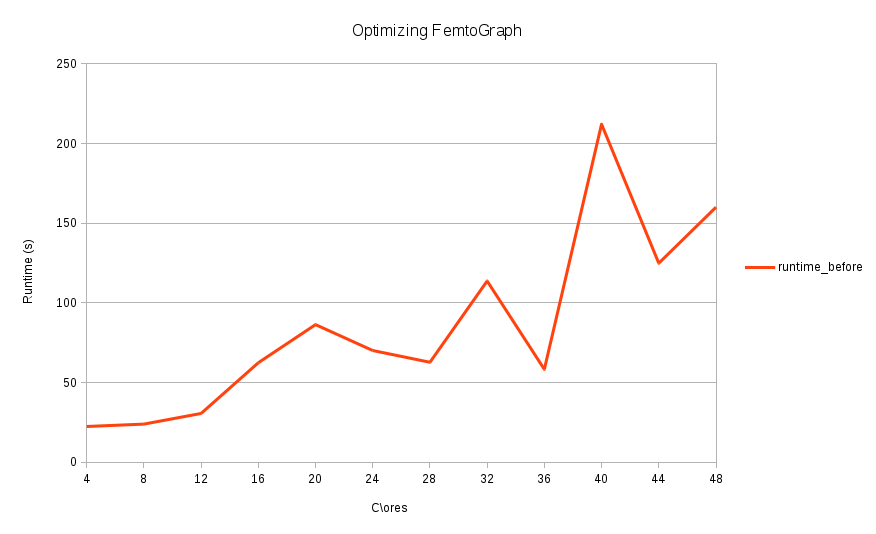
\includegraphics[width=\columnwidth]{before.png}
  \caption{Scaling before optimization}
\end{figure}


\section{Solution}
\justify
My main solution for the message queue was to use a vector of boost lockfree queues for the message queue. The vector was used to presort messages by vertex in order to minimize compute time sorting message when they were received. Adding new vertices still requires a mutex, as the vector is not lockfree. This mutex is not a problem for the algorithms that I tested, as they spend most of their time updating current vertices. The lockfree queues minimize the total bottleneck in the message queue.

Load balancing issues were solved partially by making sure that vertices were evenly divided between threads at thread start time. There was no easy way to migrate vertices between threads, but the performance loss of a single misplace vertex is trivial.  

\begin{figure}
  \centering
  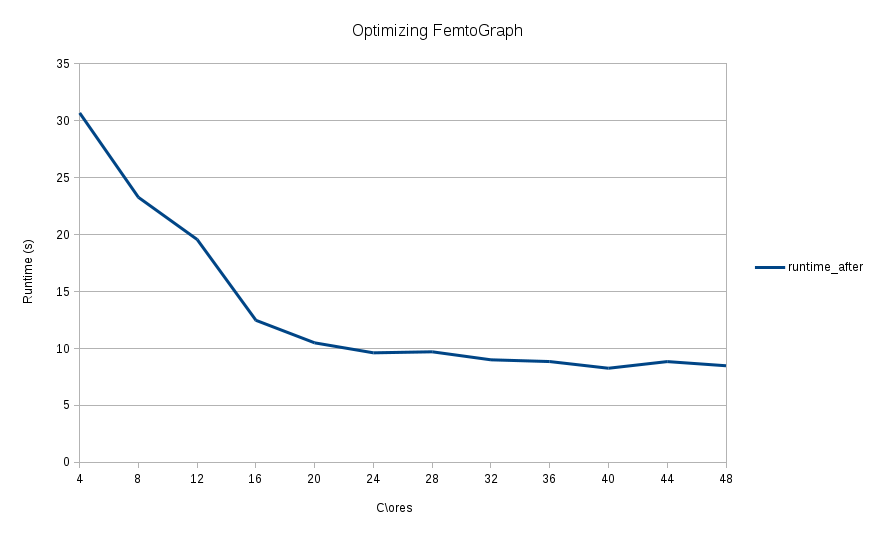
\includegraphics[width=\columnwidth]{after.png}
  \caption{Scaling after optimization}
\end{figure}



\section{Results}
\justify
We compared FemtoGraph and  GraphLab on running pagerank on a large Stanford SNAP graph. The graph used was the Wikipedia Talk Network, a directed graph based off of discussion about Wikipedia article edits with 2394385 Vertices and 5021410 edges. \cite{snapnets} The final version of FemtoGraph is capable of scaling to 48 cores on a single large system. At 28 cores, it begins to overtake graphlab in terms of runtime. In the case of both applications, only compute time was counted. reading in data and initializing graphs were outside of the measured data. 
\begin{figure}
  \centering
  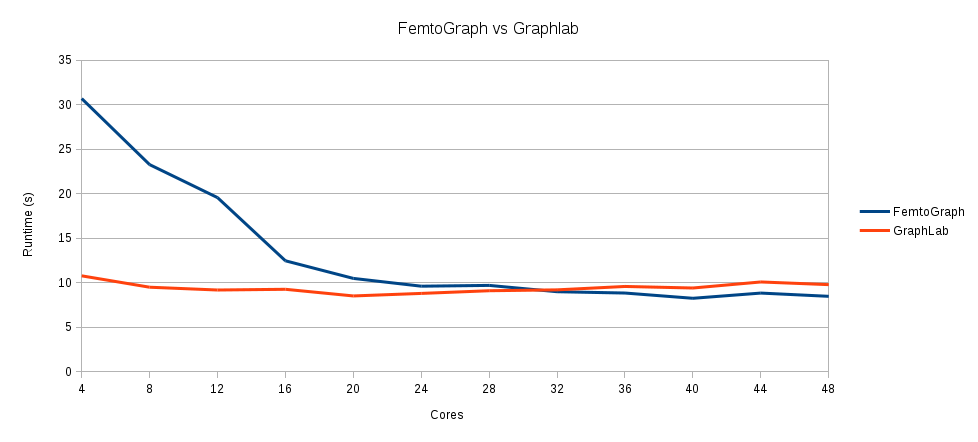
\includegraphics[width=\columnwidth]{vs.png}
  \caption{Scaling vs. GraphLab}
\end{figure}


\justify
\section{Conclusion}
FemtoGraph is a lightweight, single node graph processing system capable of scaling to large core counts and outperforming some of the current graph processing standards. FemtoGraph shows that the pregel model performs well under shared memory situations at scale.

 
% The following two commands are all you need in the
% initial runs of your .tex file to
% produce the bibliography for the citations in your paper.
\bibliographystyle{abbrv}
\bibliography{sigproc}  % sigproc.bib is the name of the Bibliography in this case
% You must have a proper ".bib" file
%  and remember to run:
% latex bibtex latex latex
% to resolve all references
%
% ACM needs 'a single self-contained file'!
%
%Appendix A
%\balancecolumns % GM June 2007
% That's all folks!
\end{document}
